%\newpage
%\subsection{Dataset}

Next, we apply our method to brain imaging data from the anonymized multimodal
neuroimaging ``Mother Of all Unification Studies'' (MOUS) dataset
\citep{schoffelen2019204}.  The dataset contains magneto-encephalography (MEG)
recordings of 102 healthy native-Dutch adults who participated in a reading
task.
%
Subjects were exposed to a rapid serial visual presentation of Dutch words. The
word lists consisted of 120 sentences, and scrambled lists of the same words.
Each word was presented on the computer screen for 351ms on average (min: 300ms,
max: 1400ms).  Successive words were separated by a blank screen for 300ms, and
successive sentences were separated by an empty screen for a few (3-4) seconds.

\subsubsection{MEG preprocessing}

The raw MEG data was bandpass-filtered between 0.1 and 40Hz using MNE-Python
default parameters \citep{gramfort2013meg, gramfort2014mne}. Specifically, we used a zero-phase finite impulse
response filter (FIR) with a Hamming window and with transition bands of 0.1Hz
and 10Hz for the low and high cut-off frequencies respectively.

The raw data was then segmented 100ms before word onset and 1.000 sec after
word onset. Time $t=0$ms corresponds to the word onset. Finally, each resulting
segment was baseline-corrected between -100ms and 0ms, and decimated by 5 and
thus led a sampling frequency of 240Hz. Figure \ref{fig:megavg} shows
the average response of the magnetometers evoked by the words presented to the
first subject.

For each subject and each time sample relative to word onset, we
build an observation matrix $Y \in \mathbb{R}^{n, q}$ of $n\approx$ 2700 words
by $q=301$ MEG channels (273 magnetometers and 28 compensation channels). Each
of the columns of $Y$ is normalized to have zero mean and unit variance.

\begin{figure}
  \centering
  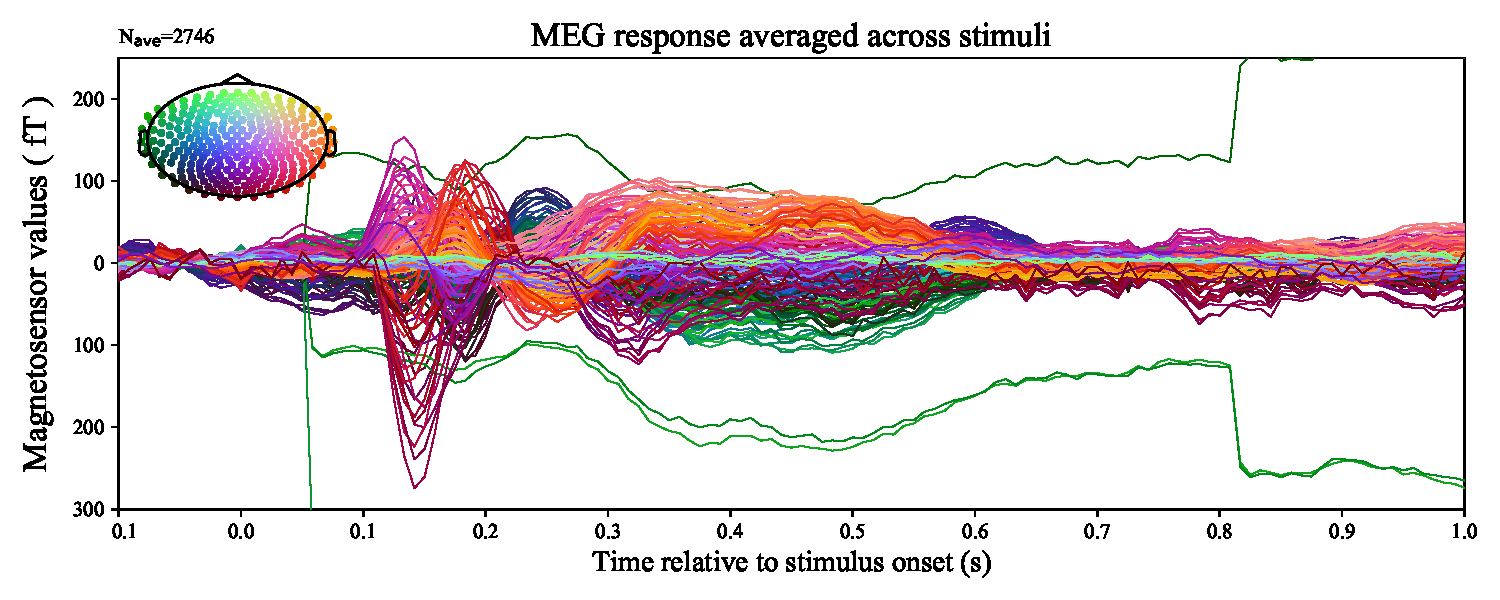
\includegraphics[width=\textwidth, trim=0cm 0cm 0cm 0cm, clip=True]{figures/meg_sensors.pdf}
  \caption{Magnetosensor response (femtoteslas fT) averaged across words for the first subject. The color coding corresponds to the positions of the sensors on the head as shown on the top-left diagram. The diverging curves correspond to artifacts in data collection.}
  \label{fig:megavg}
\end{figure}

\subsubsection{Word features} We annotated each word with 38 features: 26
correspond to the count of each letter in the word (from 'a' to 'z',
independently of their case), the total number of letters ('word length'), the
frequency of the word in natural language (using the Zipf logarithmic scale
of \citep{van2014subtlex}), and the part-of-speech tags (i.e. NOUN, PROPN (proper
noun), VERB, PRON (pronoun), CONJ (conjunction), DET (determinant), ADJ
(adjective), ADV (adverb), and NUM (numerical)) using the packages Spacy
\citep{spacy2} and WordFreq \citep{speerwordfreq}. For clarity purposes, we refer to these
features using two broad categories: visual (i.e. each letter and the total
number of letters) and lexical (part-of-speech and word frequency).  This
procedure yields an $X \in \mathbb{R}^{n, d}$ matrix of $n\approx$ 2700 words by
$d=38$ features for each subject. Each of the columns of $X$ is normalized to
have a mean and a standard deviation of 0 and 1 respectively.

\subsubsection{Methods}

We attempt to identify which factors of $X$ explain the MEG
recordings $Y$ at each time sample and for each subject separately. To this aim,
we compare three methods (forward, backward and back-to-back
regressions). Corresponding results can be found in Figure \ref{fig:meg_twocurves}.


\begin{figure}[t!]
  \centering
  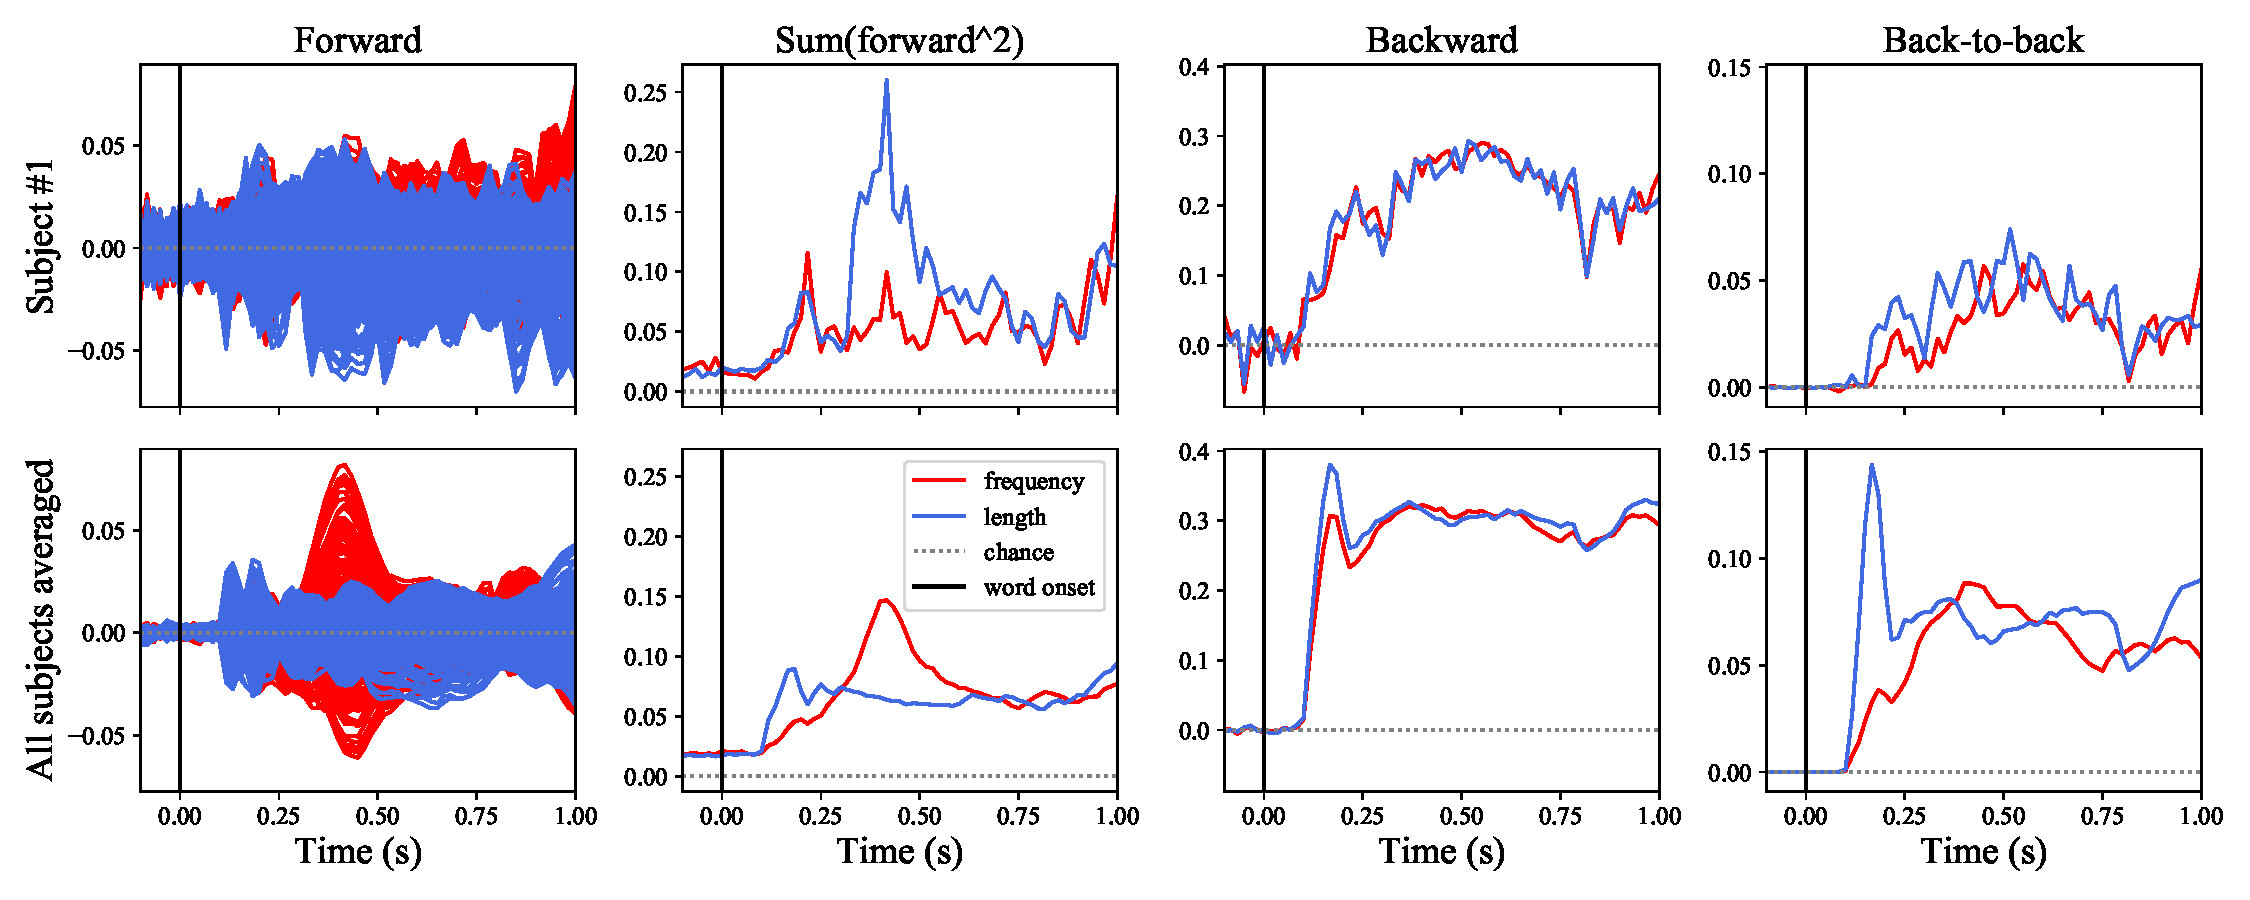
\includegraphics[width=\textwidth, trim=0cm 0cm 0cm 0cm, clip=True]{figures/meg_twocurves.pdf}
  \caption{We compare the encoding approach (columns 1 and 2, ridge regression $X \rightarrow Y$) and the decoding approach (column 3, ridge regression $Y \rightarrow X$) to our method (column 4, $X \rightarrow Y \rightarrow X$) on real MEG data from the MOUS dataset. Top row: the first subject. Bottom row: average across subjects.
  We plot the contributions of the \textit{word frequency} and the \textit{word
  length} over time. Our method can disambiguate them consistently with
  previous neuroscientific work showing an early response ($\approx$ 150ms) to
  length and a later response ($\approx$ 400ms) to frequency.}
  \label{fig:meg_twocurves}
\end{figure}

Forward regression performs a regularized least-squares regression $A \in \mathbb{R}^{d_x \times d_y}$ from $X$ to $Y$, and estimates the causal influence $E_{i,i}$ as $\| A_{i, :} \|^2$.
%
Backward regression performs a regularized least-squares regression $B \in \mathbb{R}^{d_y \times d_x}$ from $Y$ to $X$, and estimates the causal influence $E_{i, i}$ as the Pearson correlation between the $i$-th column of $X$ and the $i$-th column of $YB$, using a validation sample.
%


% \paragraph{Forward regression} also known as 'encoding' in neuroimaging, here consists of
% fitting a ridge-regularized ordinary least squares (OLS) regression \footnote{We use scikit-learn \citep{sklearn}.} from $X$ to $Y$:
% \begin{equation}
%   H = (X^{T}X+\lambda I)^{-1} X^{T}Y
% \end{equation}
% where $\lambda$ is the
% regularization parameter, cross-validated between $10^{-5}$ and $10^5$.
% 
% We then estimate the contribution
% $diag(\hat E) \in\mathbb{D}^{d} $ of each factor. However, $H\in\mathbb{R}^{d,
% q}$ is a matrix of $d$ word features by $q$ MEG channels. We approximate
% the relative contribution of each feature with the sum-of-squares of the corresponding coefficients in $H$; for the $j$-th feature:
% \begin{equation}
%   \hat e_j = \sum_{i=0}^{q} {h_{i,j}}^2
% \end{equation}
% \paragraph{Backward regression} or 'decoding', is similar but predicts $X$ from $Y$:
% \begin{equation} G = (Y^{T}Y+\lambda I)^{-1} Y^{T}X \end{equation}
% where $\lambda$ is cross-validated as for encoding. We estimate the
% contribution $diag(\hat E) \in\mathbb{D}^{d} $ of each factor in the following
% way. We predict $X$ on a held-out split \textit{test}:
% % Using 10-fold cross-validation, we thus assessed the ability of this ridge
% % regression to predict independent and identically distributed data:
% \begin{equation} \hat X_{test} = Y_{test}\cdot G_{train} \end{equation}
% and assess, for each factor of X independently, the Pearson correlation
% coefficient $r$ between $X_{test}$ and $\hat X_{test}$. We repeat the procedure
% for 20 random splits and average the result.

\paragraph{Back-to-back regression} We adapted back-to-back regression with two
changes. First, to avoid getting a slightly positively-biased estimate of the
factors contributing to the MEG signal, we swap the Tikhonov regularization of
the first regression $G$ with a truncated regularization. Truncation was fitted
 by maximum likelihood estimate, as implemented in scikit-learn principal
 component analysis. Second, to minimize the variance increase induced by
 bagging, we computed the inverse regularized covariance matrices outside
 bagging:
\begin{equation}
  G = (Y^T Y+\lambda_Y I)^{-1} Y_{train}^T X_{train}
\end{equation}
\begin{equation}
\hat X_{test} = Y_{test} \cdot G^T
\end{equation} where $\left(train,test\right)$ are partitions of the data.

\subsubsection{Second-level statistics}

The three types of analyses were implemented for each subject and each time
sample independently.  To estimate the reliability of these estimates in the
population, we tested, using one-sample $t$-test whether the distribution of
the estimated contribution of each factor different from baseline ($t=-100$ms),
as $\text{t-test}(\hat E_{t=-100} - \hat E_{\tau})$, with $\tau \in $ 150ms and
400ms respectively


\subsubsection{Results}

We aimed to estimate

We show these coefficients as a function of time in the stacked plots, in Figure
\ref{fig:megresult}.

\begin{figure}
  \centering
  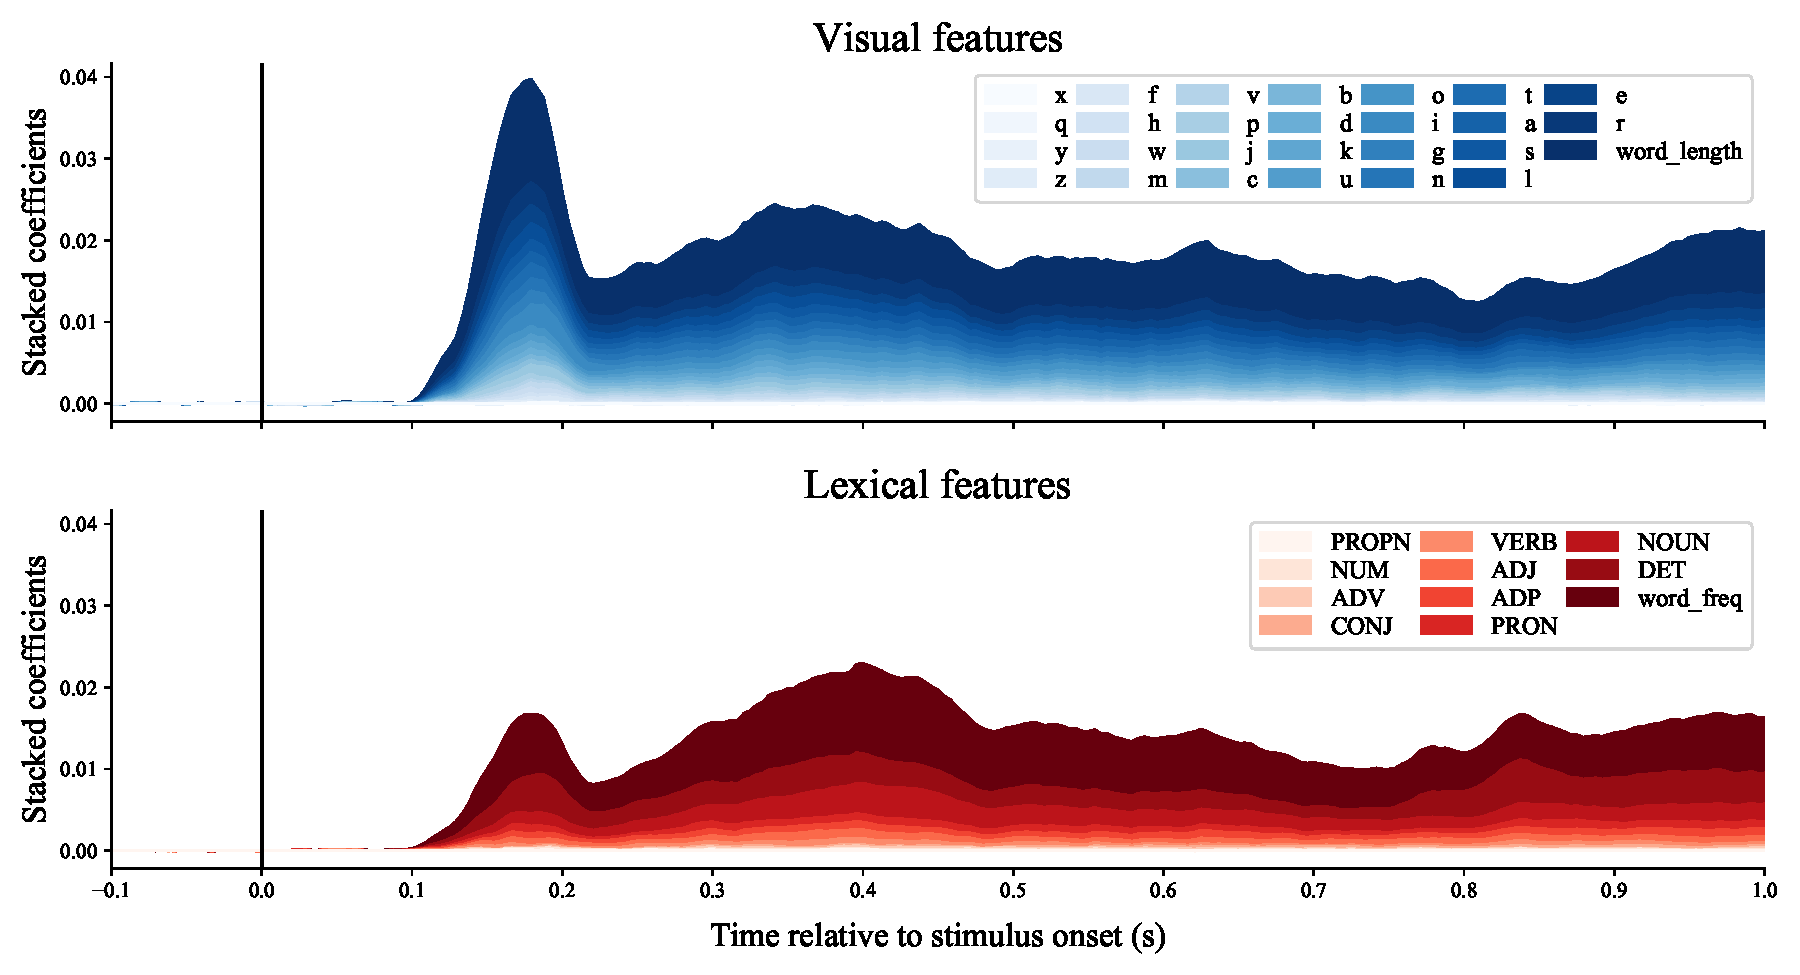
\includegraphics[width=\textwidth, trim=0cm 0cm 0cm 0cm, clip=True]{figures/meg_result.pdf}
  \caption{Average magnetosensor response across words for one subject.}
  \label{fig:megresult}
\end{figure}
